% !TEX encoding = UTF-8 Unicode

\section{\large Empirical Analysis}

%%%%%%%%%%%%%%%%%%%%

\subsection{Settings}

\begin{frame}[fragile,t]{Settings}
	\begin{itemize}\vspace{0.4mm}
	\item Stock returns conditional on the market states are normally distributed.
	\item Both Chinese and U.S.\.markets have and only have three hidden states,
        namely bear, intermediate and bull:
        \begin{enumerate}
        \item \textbf{Bear} means relatively low returns with high volatilities.
        \item \textbf{Intermediate} means returns and volatilities bot close to zero.
        \item \textbf{Bull} means relatively high returns with high volatilities.
        \end{enumerate}
        The number of hidden states is now artificially given and 
        will be analyzed and validated later.
    \item Some conjectures:
    	\begin{enumerate}
        \item Time lag effects exist and worsen due to too much weight of outdated information.
        \item Results may vary with observation periods and frequencies.
        \end{enumerate}
	\end{itemize}
\end{frame}

%%%%%%%%%%%%%%%%%%%%

\subsection{Chinese CSI 300 Index daily return series}

\subsubsection{Data Description}

\begin{frame}[fragile,t]{Chinese CSI 300 Index daily return series}
	\begin{figure}[!hbt]
    \center
    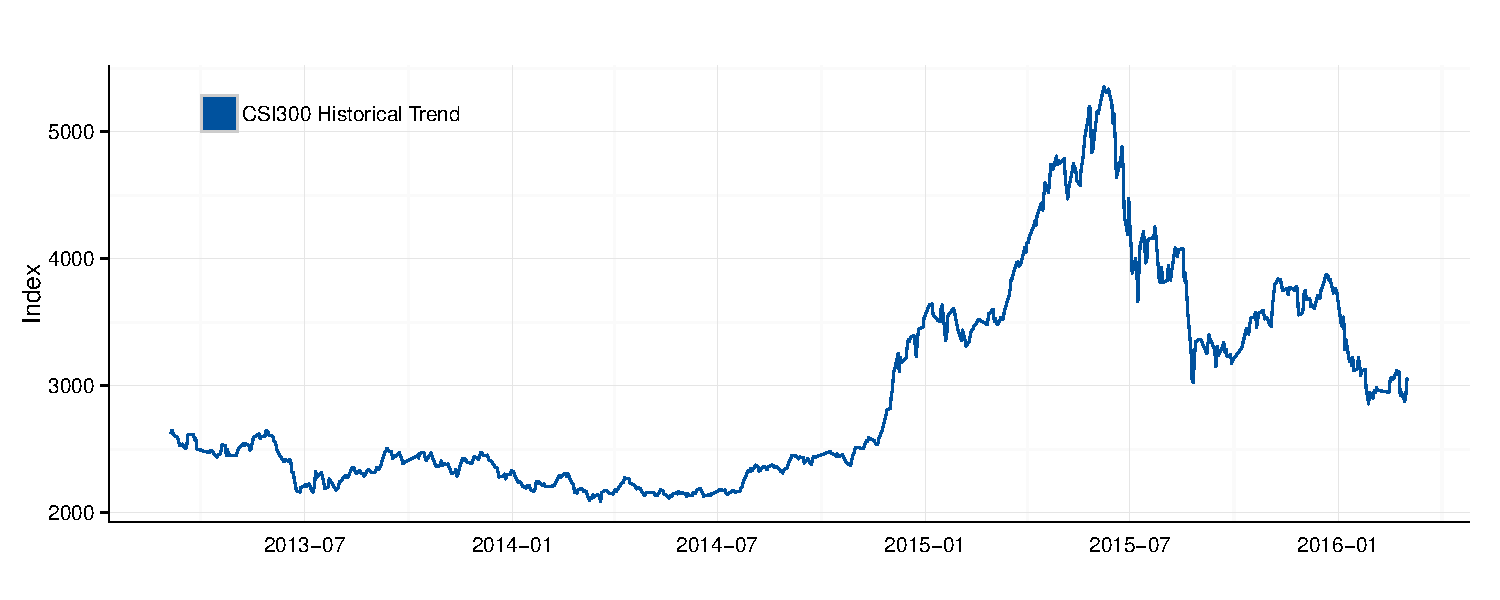
\includegraphics[width=0.8\textwidth]{daily/histFig1.pdf}
    \caption{CSI 300 historical prices}
    \label{fig:CSI:hist}
    \end{figure}

    \begin{itemize}
	\item Data range from Mar.\,$5^{th}$, 2013 to Mar\,$3^{rd}$, 2016, 
		729 prices within three years in total.
	\end{itemize}
\end{frame}

\subsubsection{Global Decoding Results}

\begin{frame}[fragile]{Chinese CSI 300 Index daily return series}
	\begin{figure}[!hbt]
    \center
    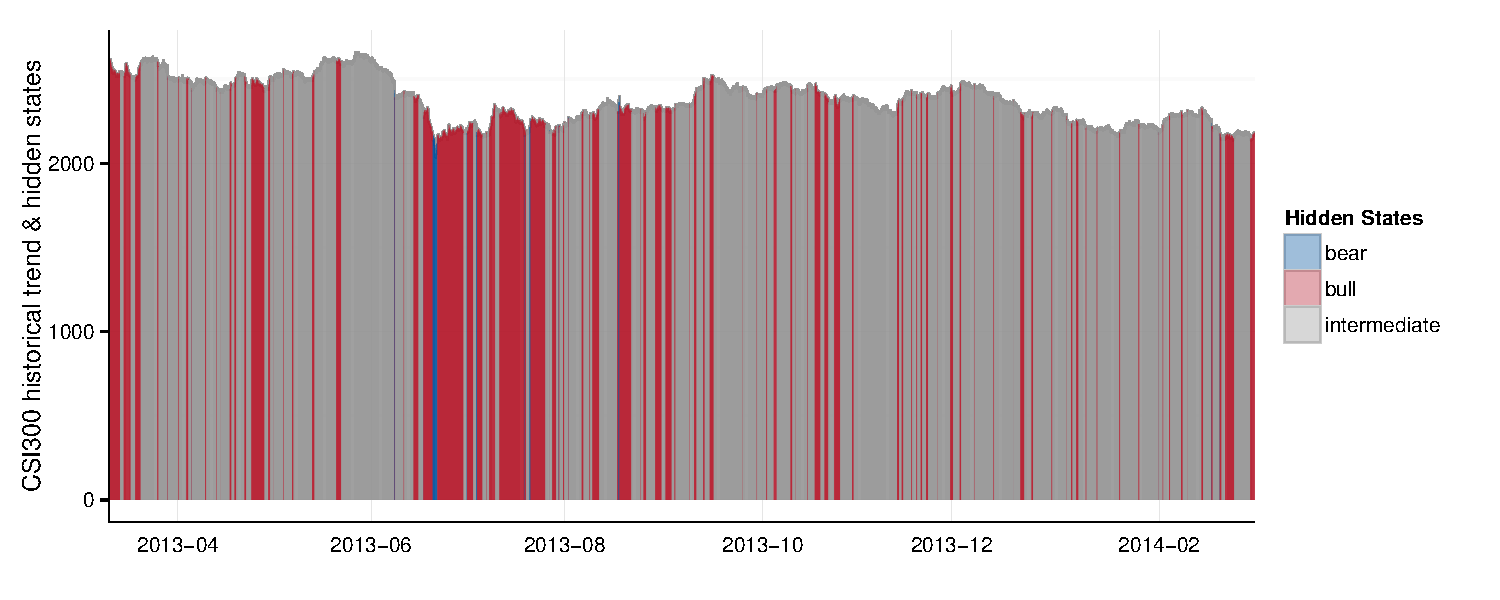
\includegraphics[width=\textwidth]{daily/statesFig1.pdf}
    \caption{CSI 300 in-sample trend and states sequence}
    \label{fig:CSI:seqstates}
    \end{figure}
\end{frame}

\begin{frame}[fragile]{Chinese CSI 300 Index daily return series}
	\begin{figure}[!hbt]
    \center
    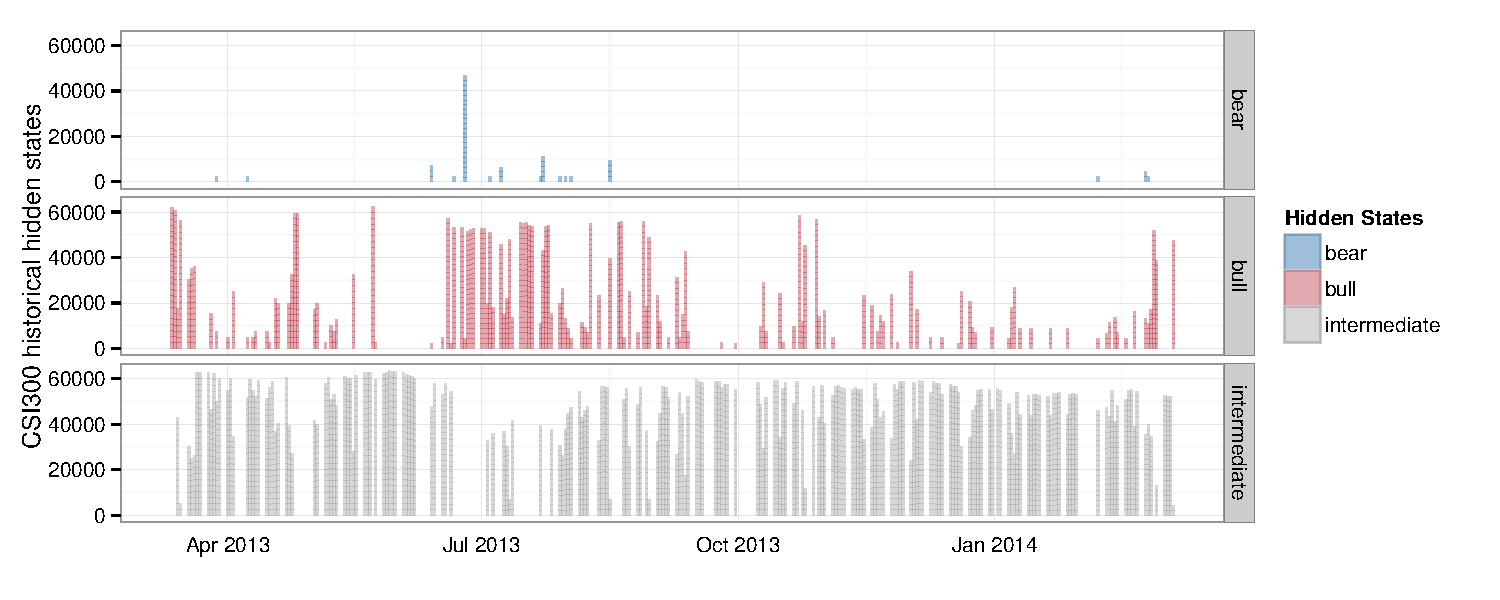
\includegraphics[width=\textwidth]{daily/statesFig2.pdf}
    \caption{CSI 300 historical hidden states}
    \label{fig:CSI:states}
    \end{figure}
\end{frame}

\subsubsection{State Transition Matrix}

\begin{frame}[fragile,t]{Chinese CSI 300 Index daily return series}
	\begin{figure}[!hbt]
    \center
    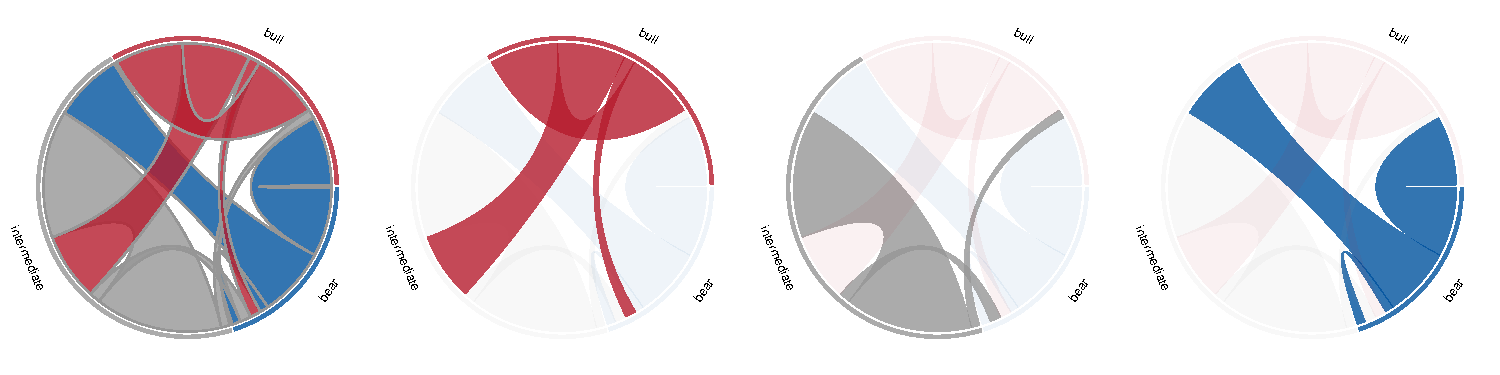
\includegraphics[width=\textwidth]{daily/transFig1.pdf}
    \caption{State transition for CSI 300 in-sample data}
    \label{fig:CSI:transition}
    \end{figure}

    \only<1>{
    \vspace*{-0.1cm}
    \begin{itemize}
	\item Colored chords start from the (same) color to another color 
		represent the transition probabilites.
	\item The thickness of the chords represent the relative relationships among the probabilities.
	\end{itemize}}
	\only<2>{
	\begin{exampleblock}{Example (Part 1 \& 2 of Fig.\,\ref{fig:CSI:transition})}
	There is a red chord starting from bull (red) and ending with intermediate (grey). 
	It represents the probability that the bull transits into the intermediate.
	Red to grey is the thickest, meaning it is most likely for bull to go into the intermediate.
	\end{exampleblock}}
\end{frame}

\begin{frame}[fragile]{Chinese CSI 300 Index daily return series}
	\begin{figure}[!hbt]
    \center
    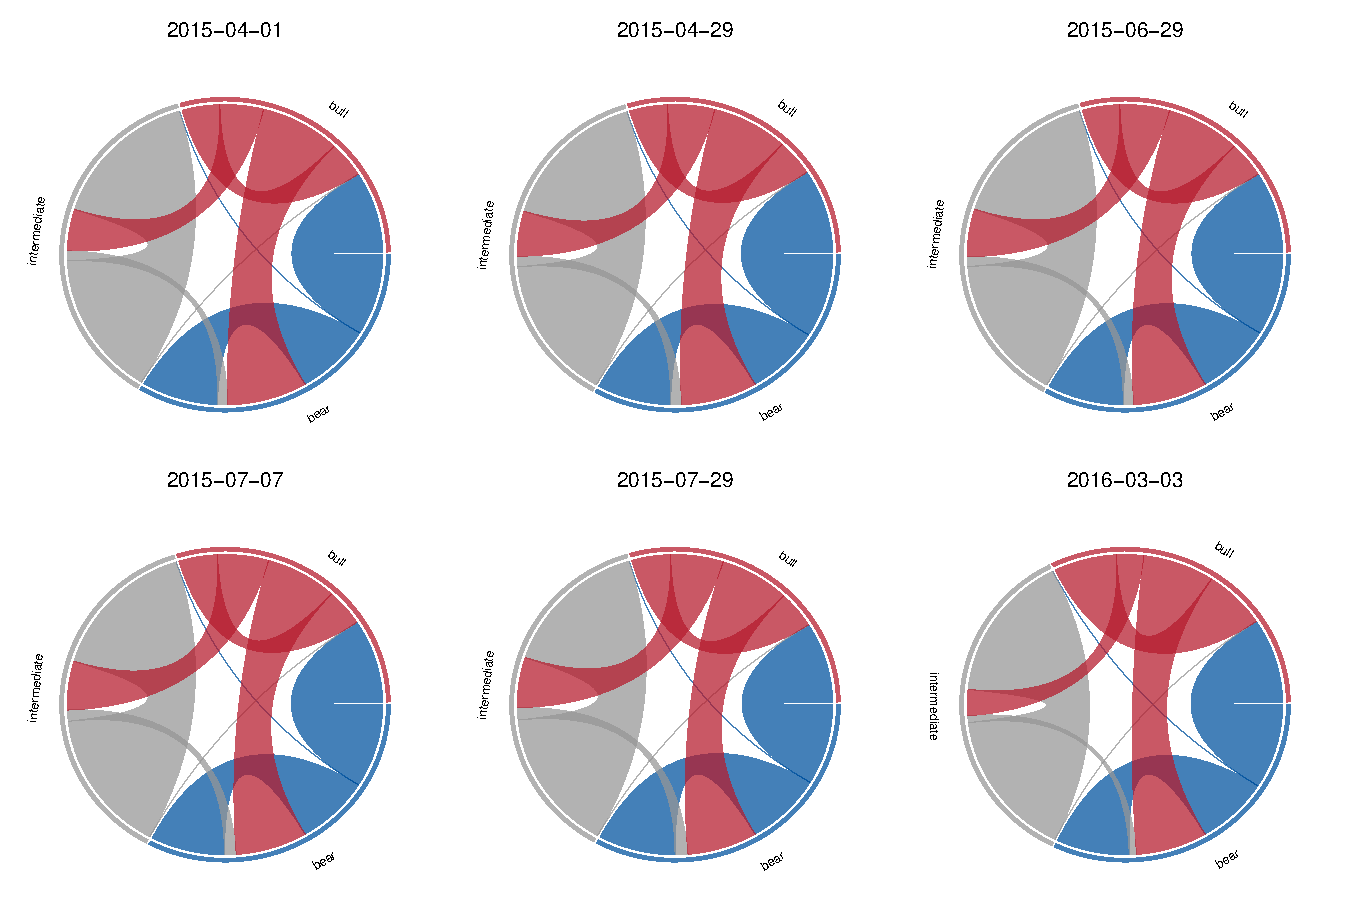
\includegraphics[width=0.75\textwidth]{daily/transFig3.pdf}
    \caption{Typical state transition matrices during the entire period }
    \label{fig:CSI:transitiontypical}
    \end{figure}
\end{frame}

\subsubsection{Conditional Distribution Parameters}

\begin{frame}[fragile,t]{Chinese CSI 300 Index daily return series}
	\begin{figure}[!hbt]
    \center
    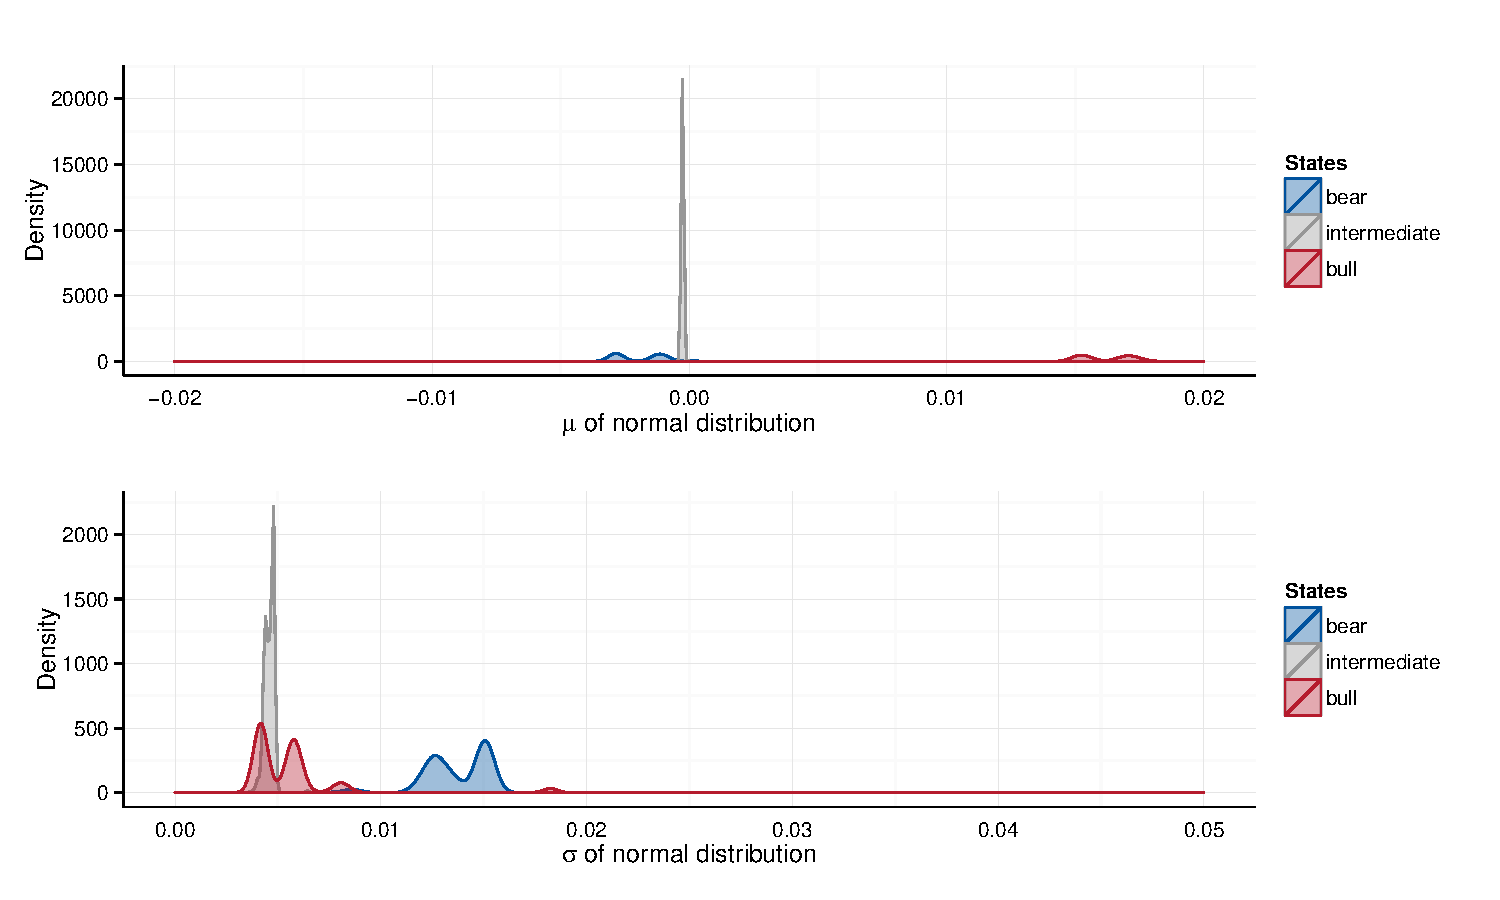
\includegraphics[width=0.72\textwidth]{daily/paramFig2.pdf}
    \caption{Density distribution of conditional distribution parameters}
    \label{fig:CSI:distdist}
    \end{figure}

    \vspace*{-1em}
	\begin{itemize}
	\item Conditional distribution parameters change with time goes by.
	\end{itemize}   
\end{frame}

\subsubsection{Simulated Predictions}

\begin{frame}[fragile,t]{Chinese CSI 300 Index daily return series}
	\begin{figure}[!hbt]
    \center
    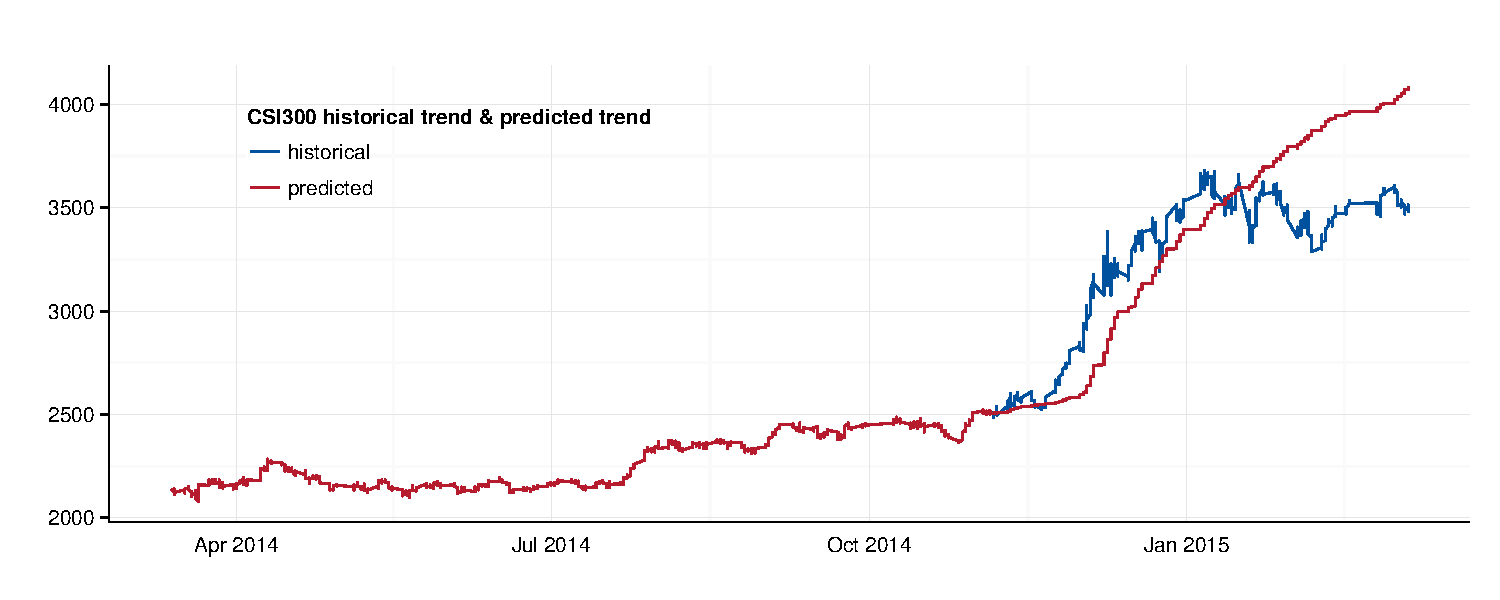
\includegraphics[width=\textwidth]{daily/predictionFig1.pdf}
    \caption{CSI 300 simulated prediction result}
    \label{fig:CSI:predictionall}
    \end{figure}

    \begin{itemize}
	\item Errors accumulate for long-period static predictions and time lag effects exist.
	\end{itemize}   
\end{frame}

\begin{frame}[fragile]{Chinese CSI 300 Index daily return series}
	\begin{figure}[!hbt]
    \center
    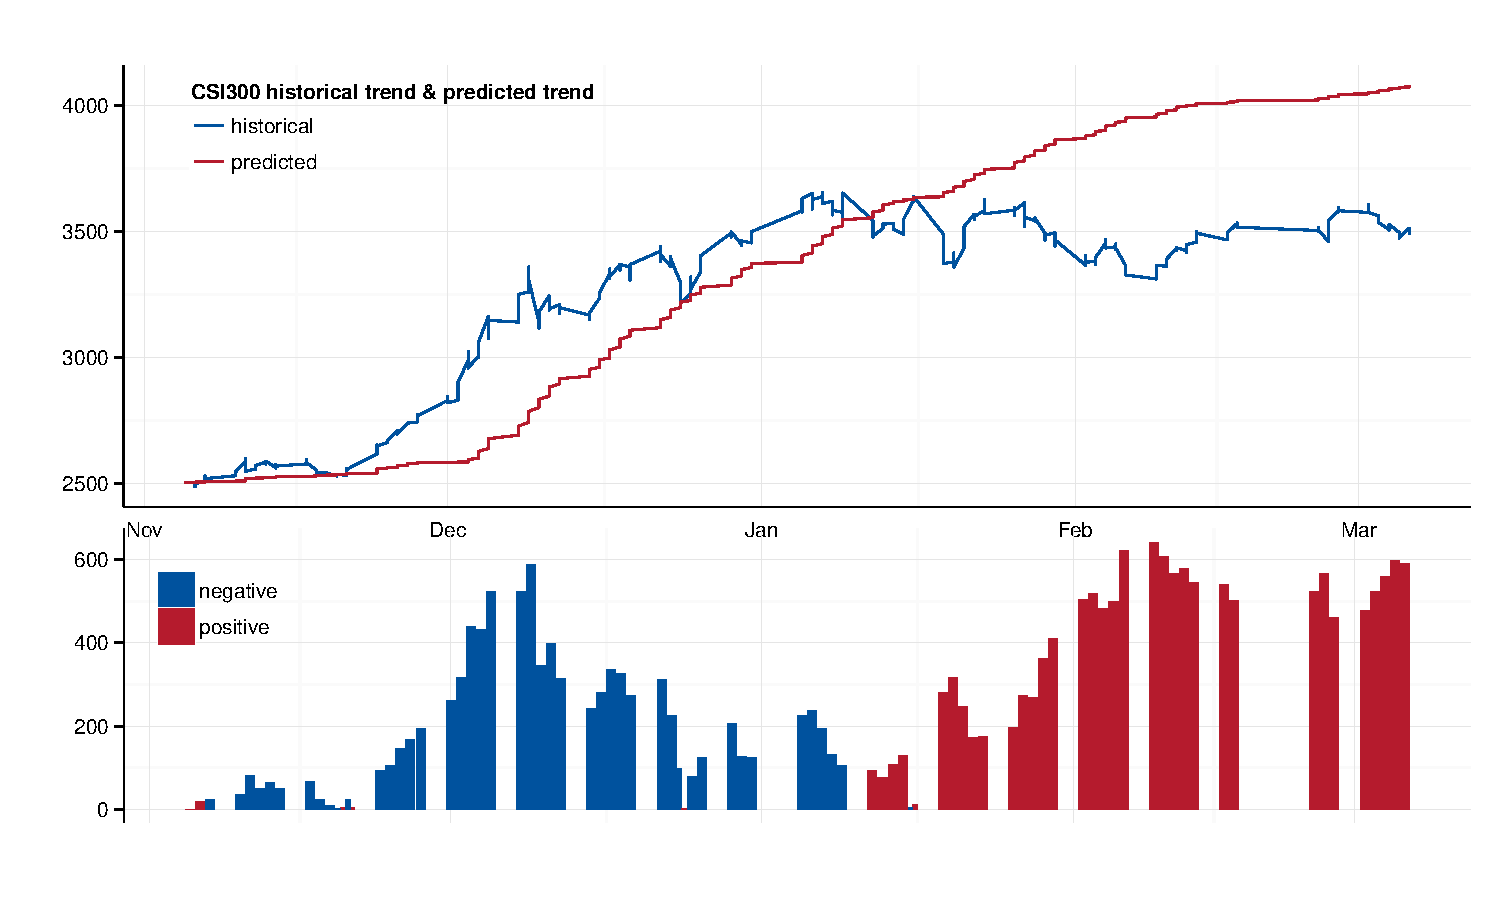
\includegraphics[width=0.8\textwidth]{daily/predictionFig2.pdf}
    \caption{CSI 300 simulated prediction result out-of-sample part}
    \label{fig:CSI:predictionout}
    \end{figure}
\end{frame}

\begin{frame}[fragile]{Chinese CSI 300 Index daily return series}
	\begin{figure}[!hbt]
    \center
    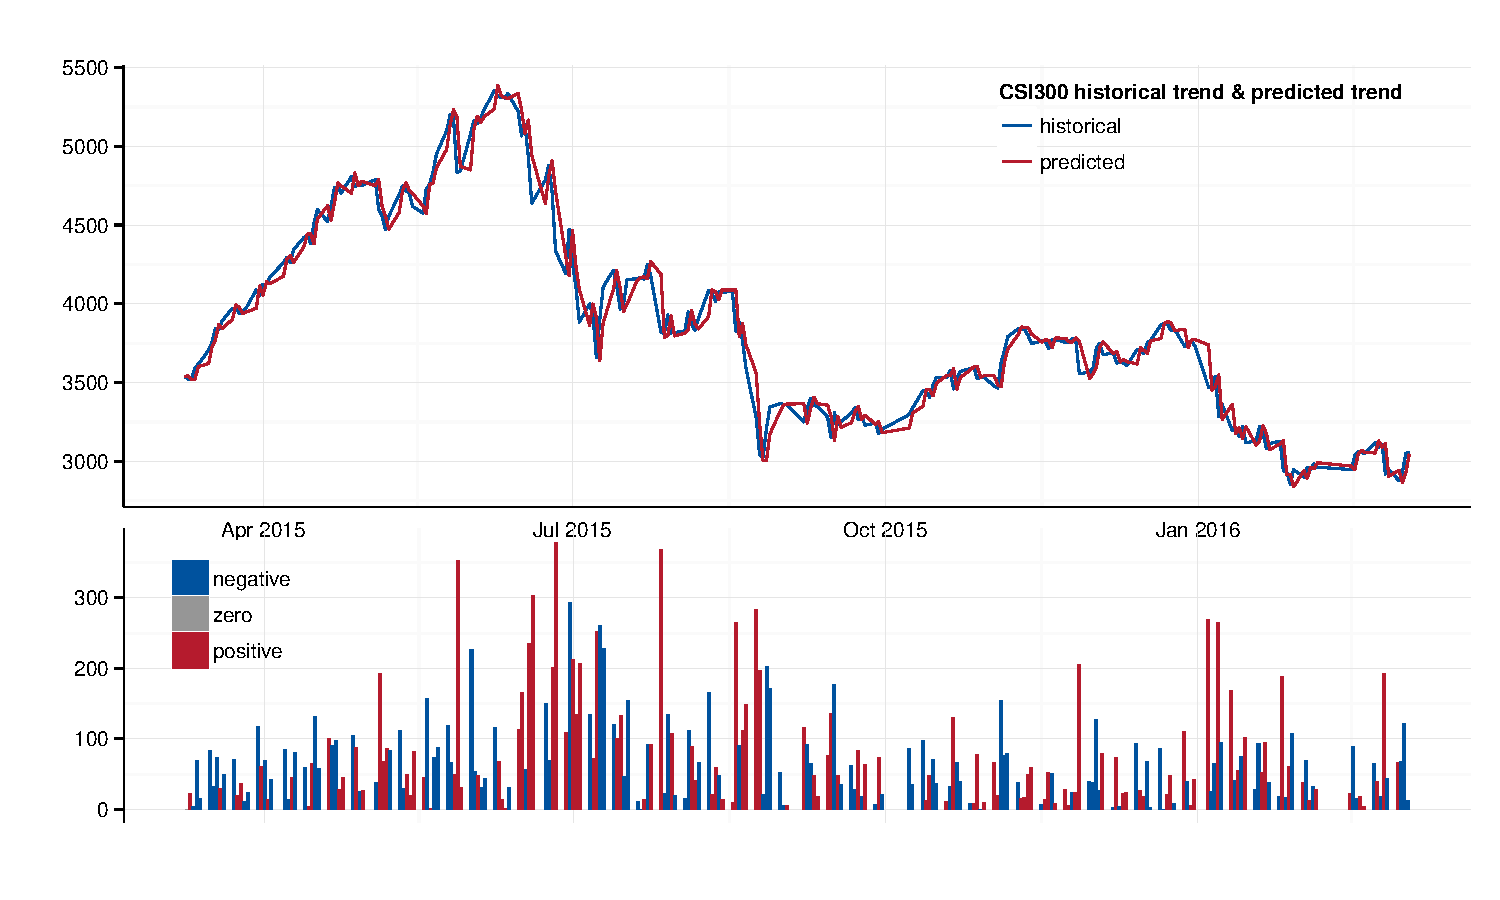
\includegraphics[width=0.8\textwidth]{daily/predictionFig4.pdf}
    \caption{CSI 300 adaptive predictions}
    \label{fig:CSI:adaptive}
    \end{figure}
\end{frame}

\begin{frame}[fragile,t]{Chinese CSI 300 Index daily return series}
	\begin{figure}[!hbt]
    \center
    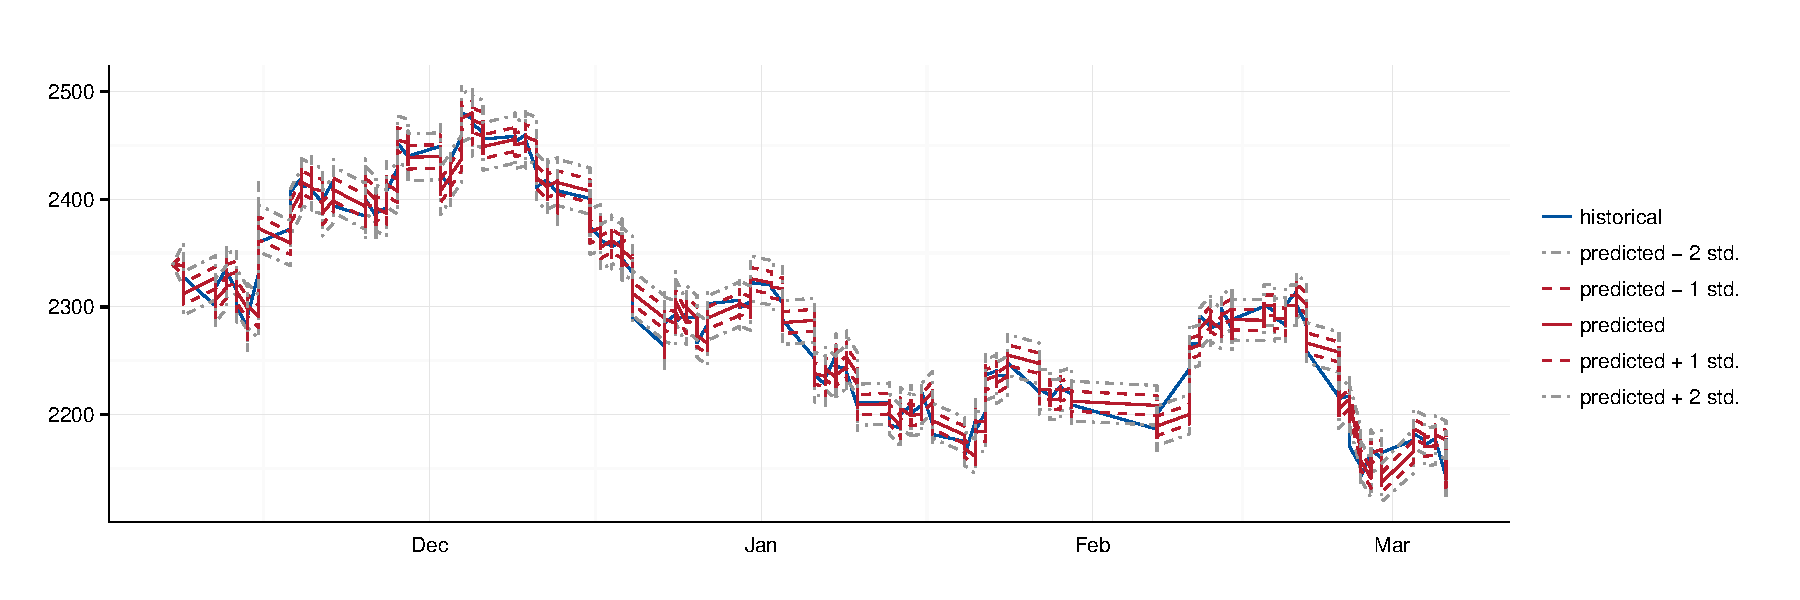
\includegraphics[width=\textwidth]{daily/predictionFig5.pdf}
    \caption{CSI 300 adaptive predictions with confidence interval}
    \label{fig:CSI:adaptiveconfi}
    \end{figure}

    \begin{itemize}
	\item All actual historical returns are within two standard deviations from the predicted return,
		and thus the adaptive predicted price level.
	\end{itemize}   
\end{frame}

%%%%%%%%%%%%%%%%%%%%

\subsection{The Number of Hidden States}

\begin{frame}[fragile,t]{The Number of Hidden States}
	\begin{figure}[!hbt]
    \begin{center}
    \subfigure[AIC vs. N]
        {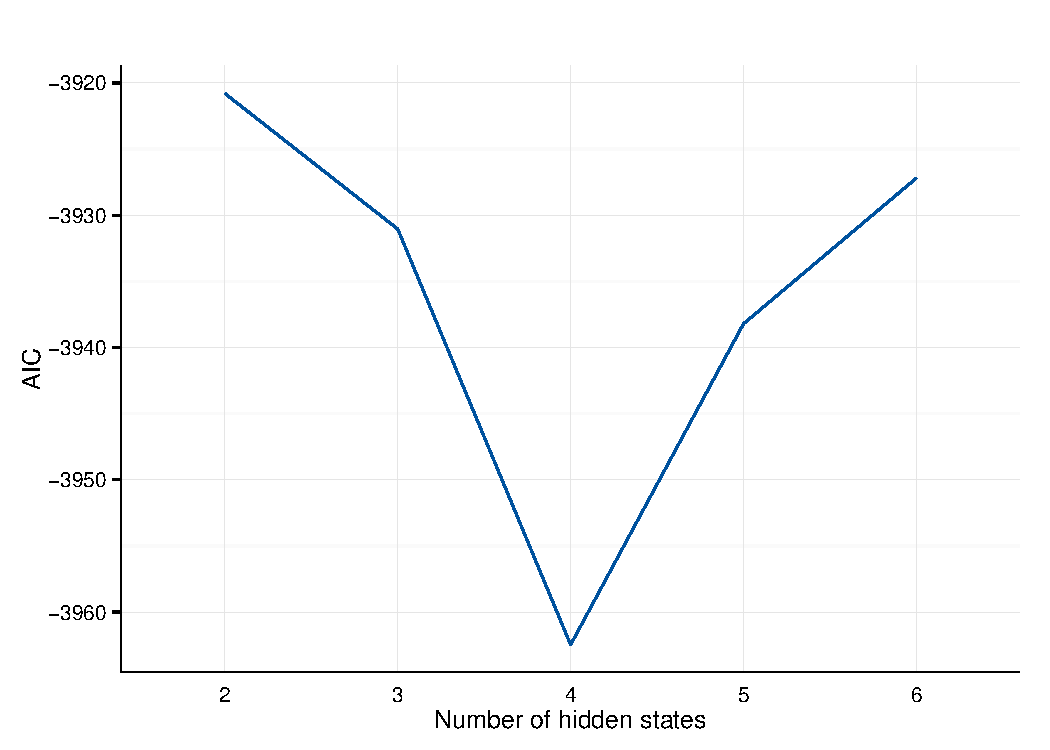
\includegraphics[width=0.45\textwidth]{states/numStateAIC.pdf}}
    \subfigure[BIC vs. N]
        {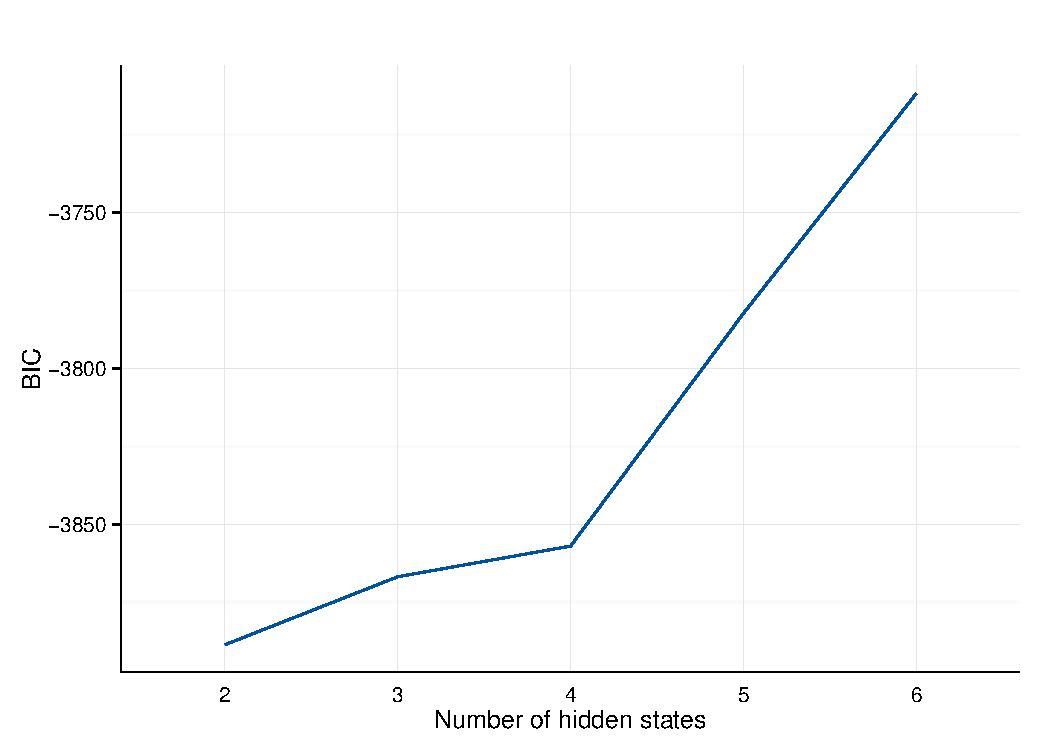
\includegraphics[width=0.45\textwidth]{states/numStateBIC.pdf}}
    \end{center}
    \caption{Goodness of fit for different number of hidden states}
    \label{fig:result:states}
    \end{figure}

    \vspace*{-1em}
    \begin{itemize}
	\item Four is optimal from AIC and two from BIC, so three is reasonable.
	\end{itemize}
\end{frame}

%%%%%%%%%%%%%%%%%%%%

\subsection{Prediction Results Summary}

\begin{frame}[fragile]{Prediction Results Summary}
	\begin{table}[!hbt]
    \center
    \caption{Brief description of all prediction results}
    \label{table:results}
    \begin{tabular}{c c c c c}
    \hline
    Target Index  &  Data Frequency  &  Time Period  &  Data Length  &  Win Ratio  \\
    \hline
    S\&P 500  &  daily  &  2013$\sim$2016  &  757  &  50.4\%  \\
    CSI 300   &  daily  &  2013$\sim$2016  &  729  &  50.2\%  \\
    CSI 300   &  60min  &  2013$\sim$2014  &  968  &  51.7\%  \\
    CSI 300   &  60min  &  2014$\sim$2015  &  976  &  55.5\%  \\
    CSI 300   &  60min  &  2015$\sim$2016  &  972  &  50.5\%  \\
    CSI 300   &  10min  &  2013$\sim$2014  &  5808  &  51.7\%  \\
    CSI 300   &  10min  &  2014$\sim$2015  &  5856  &  57.5\%  \\
    CSI 300   &  10min  &  2015$\sim$2016  &  5832  &  52.0\%  \\
    \hline
    \end{tabular}
    \end{table}
\end{frame}
